\documentclass[../main.tex]{subfiles}
\begin{document}
\chapter{Central Forces}
An important class of potentials depend only on the distance to some origin.
For example in \cref{gravity}, we saw that the force one one mass depends on its radial distance to another mass, so, if we treat the other mass s the origin, the force on the first particle depends only on its distance $r$ to that origin.
Similarly, in \cref{electricForces}, we saw that the force on one charge depends on its radial distance to another charge.

We can therefore express such potentials $V$ as a function of the radial distance:
\[
  V(\vec{x}) = V(|\vec{x}|) = V(r) \text{ where $r = |\vec{x}|$}
\]
The conservative force (\cref{conservativeForce}) associated with such a potential therefore points towards, or away from, the origin:
\begin{align}
  \vec{F} &= - \nabla V(r) \nonumber \\
          &= - \deriv{V}{r} \nabla r \text{ using the chain rule} \nonumber \\
          &= - \deriv{V}{r} \uvec{x} \text{ as $\nabla r = \frac{\vec{x}}{r}$ from \cref{gravity}} \label{radialForce}
\end{align}
which either points towards or away from the origin in the direction of $\uvec{x}$.
\begin{remark}[Notation]
  Sometimes we will denote $\frac{\vec{x}}{r}$ as $\uvec{r}$ or $\vec{e}_r$ instead of $\uvec{x}$.
\end{remark}
\section{Conservation of Angular Momentum}
The most important fact about \textit{central potentials} is that \textit{angular momentum} is conserved.
\begin{definition}[Angular Momentum]
  The \textit{angular momentum} $\vec{L}$ of a particle of mass $m$ at $\vec{x}$ relative to its centre of rotation is defined to be:
  \[
    \vec{L} = m \vec{x} \times \dot{\vec{x}} = \vec{x} \times \vec{p}
  \]
\end{definition}
\begin{remark}
  $\vec{L}$ is defined relative to an origin, here we are setting the origin at $\vec{x} = \vec{0}$, however, we will generalise later.
\end{remark}
Note that the angular momentum is orthogonal to both position and momentum/velocity.
\begin{center}
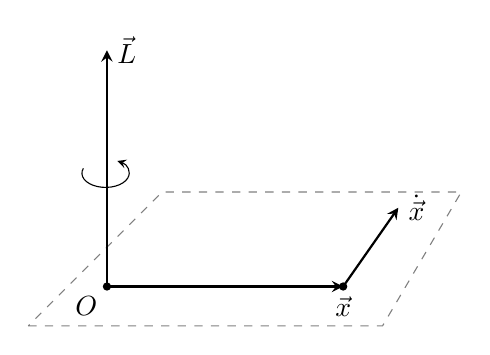
\begin{tikzpicture}[>=stealth]
  \draw[gray, dashed] (-1,-0.5) -- (3.5, -0.5) -- (4.5, 1.2) -- (0.7, 1.2) -- cycle;
  \fill (0, 0) circle (1.5pt) node[below left] {$O$};
  \draw[thick,->] (0,0) -- (3,0) node[below] {$\vec{x}$};
  \fill (3, 0) circle (1.5pt);
  \draw[thick,->] (3,0) -- (3.7,1) node[right] {$\dot{\vec{x}}$};
  \draw[thick,->] (0,0) -- (0,3) node[right] {$\vec{L}$};
  \draw[->, yscale=0.6] (-0.3,2.5) arc [start angle=-200,end angle=60,radius=0.3];
\end{tikzpicture}
\end{center}
For a general force $\vec{F}$:
\begin{align*}
  \deriv{\vec{L}}{t} &= m \deriv{}{t}(\vec{x} \times \dot{\vec{x}}) \\
                     &= m(\cancelto{\vec{0}}{\dot{\vec{x}} \times \dot{\vec{x}}} + \vec{x} \times \ddot{\vec{x}}) \\
                     &= \vec{x} \times (m \ddot{\vec{x}}) \\
                     &= \vec{x} \times \vec{F}
\end{align*}
We define the \textit{torque} to be $\vec{G} \equiv \vec{x} \times \vec{F}$.
\begin{remark}
  $\deriv{\vec{L}}{t} = \vec{G}$ is analogous to Newton's 2nd Law (\cref{newton2}), but for angular momentum.
\end{remark}
For a central force, $\vec{F} \parallel \vec{x} \implies \vec{x} \times \vec{F} = \vec{0} \implies \deriv{\vec{L}}{t} = 0$ and thus angular momentum is conserved by central forces.

Because $\vec{L}$ is a constant vector and obeys $\vec{L} \cdot \vec{x} = 0$ and $\vec{L} \cdot \dot{\vec{x}} = 0$, both the position and velocity are contained to a plane perpendicular to $\vec{L}$ and so 3D dynamics reduce to 2D dynamics on a plane.
\section{Polar Coordinates in the Plane}
\begin{definition}[Plane Polar Coordinates]
  Plane polar coordinates are defined by:
  \[
    x = r \cos \theta,\ y = r \sin \theta
  \]
  where $r \geq 0$ and $\theta$ can be restricted to $(0, 2\pi]$.
  We write the components in the order $(r, \theta)$.
\end{definition}
\begin{center}
\begin{tikzpicture}[>=stealth]
  \draw[->] (-0.5, 0) -- (3, 0) node[right] {$x$};
  \draw[->] (0, -0.5) -- (0, 3) node[above] {$y$};

  \draw[->, thick] (0, 0) -- (1.5, 1.5) node[below right] {$\vec{x}$} node[midway, above] {$r$};
  \draw (0.6,0) arc [start angle=0,end angle=45,radius=0.6] node[pos=0.7,right] {$\theta$};
  \fill (1.5, 1.5) circle (1.5pt);
  \draw[->] (1.5, 1.5) -- (1, 2) node[left] {$\uvec{\theta}$};
  \draw[->] (1.5, 1.5) -- (2, 2) node[right] {$\uvec{r}$};
\end{tikzpicture}
\end{center}
At each point, there is a local basis $\{\uvec{r}, \uvec{\theta}\}$ given in Cartesian coordinates by:
\[
  \uvec{r} = \begin{pmatrix}
  \cos \theta \\
  \sin \theta \\
  \end{pmatrix},\
  \uvec{\theta} = \begin{pmatrix}
  -\sin \theta \\
  \cos \theta \\
  \end{pmatrix}
\]
Recall from Vector Calculus that these vectors depend on position:
\[
  \deriv{\uvec{r}}{\theta} = \begin{pmatrix}
  -\sin \theta \\
  \cos \theta \\
  \end{pmatrix} = \uvec{\theta},\
  \deriv{\uvec{\theta}}{\theta} = \begin{pmatrix}
  -\cos \theta \\
  -\sin \theta \\
  \end{pmatrix}= -\uvec{r}
\]
We need to keep track of these changes when we write vector equations using polar coordinates.
We can write $\vec{x} = r \uvec{r}$ so we can differentiate to find $\ddot{\vec{x}}$:
\begin{align*}
  \dot{\vec{x}} &= \dot{r} \uvec{r} + r \dot{\uvec{r}} \\
                &= \dot{r} \uvec{r} + r \deriv{\uvec{r}}{\theta} \deriv{\theta}{t} \\
                &= \dot{r} \uvec{r} + r \dot{\theta} \uvec{\theta}
\end{align*}
$\dot{\theta}$ is often called the \textit{angular velocity}.

We can differentiate again to get $\ddot{\vec{x}}$:
\begin{align*}
  \ddot{\vec{x}} &= \ddot{r} \uvec{r} + \dot{r}\dot{\uvec{r}} + \dot{r} \dot{\theta} \uvec{\theta} + r(\ddot{\theta}\uvec{\theta} + \dot{\theta}\dot{\uvec{\theta}}) \\
                 &= \ddot{r} \uvec{r} + 2 \dot{r} \dot{\theta} \uvec{\theta} + r \ddot{\theta} \uvec{\theta} - r \dot{\theta}^2 \uvec{r} \\
                 &= (\ddot{r} - r \dot{\theta}^2)\uvec{r} + (r \ddot{\theta}  + 2\dot{r} \dot{\theta}) \uvec{\theta}
\end{align*}
\begin{example}[Circular Motion]
  Suppose we have circular motion at a constant angular velocity $\omega$.
  We then have $\dot{r} = 0,\ \ddot{r} = 0$ and $\dot{\theta} = \omega,\ \ddot{\theta} = 0$.
  Even though both $\ddot{r}$ and $\ddot{\theta}$ are 0, this does not mean that the particle is not accelerating as we see that:
  \[
    \ddot{\vec{x}} = (0 - r\omega^2)\uvec{r} + (r(0) + 2(0)(0))\uvec{\theta} =  -r \omega^2 \uvec{r}
  \]
  So we require an acceleration towards the origin and therefore a \textit{centripetal force} towards the origin.
  \begin{center}
  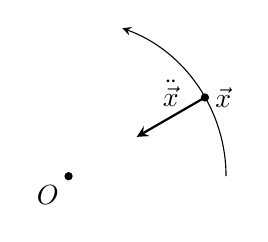
\begin{tikzpicture}[>=stealth]
    \fill (0, 0) circle (1.5pt) node[below left] {$O$};
    \draw[->] (2,0) arc [start angle=0,end angle=70,radius=2];
    \coordinate (X) at (1.732, 1);
    \draw[->, thick] (X) node[right] {$\vec{x}$} -- (0.866, 0.5) node[midway, above] {$\ddot{\vec{x}}$};
    \fill (X) circle (1.5pt);
  \end{tikzpicture}
  \end{center}
  If there was no such force, then the velocity of the particle would be constant and so it would just travel in a straight line.
\end{example}
To write Newton's second law for a central force, recall from \cref{radialForce} that $\vec{F} = -\deriv{V}{r}\uvec{r}$.
Combining this with the above, we have:
\[
  m\ddot{x} = m(\ddot{r} - r \dot{\theta}^2)\uvec{r} + m(r \ddot{\theta}  + 2\dot{r} \dot{\theta}) \uvec{\theta} = -\deriv{V}{r}\uvec{r}
\]
Since $\uvec{r}$ and $\uvec{\theta}$ form an orthonormal basis, we can equate the radial and angular components to yield:
\begin{align}
  \uvec{r}:&\ m(\ddot{r} - r \dot{\theta}^2) = -\deriv{V}{r} \label{eqnRadial} \\
  \uvec{\theta}:&\ r\ddot{\theta}  + 2\dot{r}\dot{\theta} = 0 \label{eqnAngular}
\end{align}
We can rewrite \cref{eqnAngular} as:
\begin{align*}
  \frac{1}{r}\deriv{}{t}(r^2 \dot{\theta}) &= 0 \\
  \implies r^2 \dot{\theta} &= \ell \text{ is constant}
\end{align*}
In fact, this is the magnitude of the angular momentum:
\begin{align*}
  \vec{L} = m \vec{x} \times \dot{\vec{x}} &= m r \uvec{r} \times(\dot{r} \uvec{r} + r \dot{\theta}\uvec{\theta}) \\
                                           &= m r \dot{r} \cancelto{\vec{0}}{\uvec{r} \times \uvec{r}} + mr^2 \dot{\theta} \uvec{r} \times \uvec{\theta} \\
                                           &= mr^2 \dot{\theta} \uvec{r} \times \uvec{\theta}
\end{align*}
Note that $\uvec{r}$ and $\uvec{\theta}$ are orthogonal unit vectors so their cross product is also a unit vector, thus:
\[
  |\vec{L}| = m r^2 \dot{\theta} = m \ell
\]
\begin{remark}
  We sometimes refer to $\ell$ as ``angular momentum'' despite it technically being angular momentum \textit{per unit mass}.
\end{remark}

To get rid of the $\theta$ dependence in \cref{eqnRadial}, we can substitute $\dot{\theta} = \ell/r^2$:
\begin{align*}
  m\left(\ddot{r} - r\frac{\ell^2}{r^4}\right) &= -\deriv{V}{r} \\
  m\ddot{r} &= - \deriv{V}{r} + \frac{m\ell^2}{r^3} \\
            &= -\deriv{}{r}\left(V + \frac{m\ell^2}{2r^2}\right) \\
            &= -\deriv{V_{\text{eff}}}{r}
\end{align*}
where $V_{\text{eff}} = V(r) + \frac{m\ell^2}{2r^2}$ is called the \textit{effective potential}.

So we have effectively reduced the problem in 2D plane polar coordinates down to a one dimensional problem.
This is all possible because of the conserved angular momentum.
\section{Effective Potential}
Consider $V(r) = -\frac{k}{r}$, i.e. an attractive $\frac{1}{r}$ potential (as seen for gravity in \cref{gravity}) so that:
\[
  V_{\text{eff}}(r) = -\frac{k}{r} + \frac{m\ell^2}{2r^2}
\]
We can plot the graph of this to analyse the motion in the radial direction:
\begin{center}
\begin{tikzpicture}[scale=1.13, >=stealth]
  \draw[->] (0, 0) -- (9, 0) node[right] {$r$};
  \draw[->] (0, -2) -- (0, 2) node[above] {$V_{\text{eff}}$};

  \node at (1.7, 1.5) {$\frac{m\ell^2}{2r^2}$ behaviour};
  \node at (7, -1) {$-\frac{k}{r}$ behaviour};

  \def\kconst{4.5}
  \def\mlconst{3}

  \clip (0,-2) rectangle (9,2);
  \draw[thick, domain=0.1:9, smooth, samples=100] plot (\x,{-\kconst/\x + \mlconst/(\x)^2});
  \draw[|-|, thick] (0, -0.1) -- (0.67, -0.1) node[midway, below] {\small B};
\end{tikzpicture}
\end{center}
Region $B$ above is known as the \textit{centrifugal barrier}.
In this region, the angular momentum prevents the particle from getting too close to the origin.

We can also derive the effective potential from the conserved energy:
\begin{align*}
  E &= \frac{1}{2} m \dot{\vec{x}} \cdot \dot{\vec{x}} + V(r) \\
    &= \frac{1}{2} m (\dot{r} \uvec{r} + r \dot{\theta} \uvec{\theta}) \cdot (\dot{r} \uvec{r} + r \dot{\theta} \uvec{\theta}) + V(r) \\
    &= \frac{1}{2} m (\dot{r}^2 + r^2 \dot{\theta}^2) + V(r) \text{ as $\uvec{r} \cdot \uvec{\theta} = 0$ and $|\uvec{r}| = |\uvec{\theta}| = 1$}\\
    &= \frac{1}{2} m \dot{r}^2 + \frac{1}{2} m r^2 \left(\frac{\ell}{r^2}\right)^2 + V(r) \\
    &= \frac{1}{2} m \dot{r}^2 + V(r) + \frac{m\ell^2}{2r^2} \\
    &= \frac{1}{2} m \dot{r}^2 + V_{\text{eff}}(r)
\end{align*}
The centrifugal barrier is the angular kinetic energy $\frac{1}{2}m\dot{r}^2$.
\end{document}
